\documentclass{article}

\usepackage{aistats2021_author_response}

\usepackage[utf8]{inputenc} % allow utf-8 input
\usepackage[T1]{fontenc}    % use 8-bit T1 fonts
\usepackage{hyperref}       % hyperlinks
\usepackage{url}            % simple URL typesetting
\usepackage{booktabs}       % professional-quality tables
\usepackage{amsfonts}       % blackboard math symbols
\usepackage{nicefrac}       % compact symbols for 1/2, etc.
\usepackage{microtype}      % microtypography
\usepackage{xcolor}         % define colors in text
\usepackage{xspace}         % fix spacing around commands
\usepackage{subfigure}
\usepackage{float}
\usepackage{graphicx}
\usepackage{wrapfig}

\begin{document}

We sincerely thank the five reviewers for their valuable feedback.


\vspace{0.01in}

\textbf{\textcolor{blue}{R1:}}
\textbf{Convergence Bounds:} 
We will simplify the presentation of the constants in our Theorems.
The condition on the growth of the sequence $\hat{V}$ is indeed controlled in AMSGrad thanks to the max operator and not in Adam. That is the whole point of the AMSGrad. This paper does not improve the flaw of Adam regarding that non-monotonicity point.

\textbf{Experiments:} 
Our experiments serve as a support of our theory that decentralized AMSGrad can converge while DADAM cannot.
We recall that the purpose of this paper is to provide both an \emph{algorithmic} and {theoretical} framework for decentralized variants of adaptive gradient methods. 
 Figure 1 shows the divergence issue of DADAM is negligible on homogeneous data but can be a big problem on heterogeneous data, highlighting the need for convergent algorithms in practice. 
 Exploring more benefits of the proposed algorithms is indeed an important and interesting question for practitioners. However, to be honest, the authors currently do not have enough  resources to scale up the experiments since it requires setting up a distributed computation environment on more machines and common free computation resources do not support it. 
 To the best of our knowledge, adaptive gradient methods are never used in decentralization with rigorous guarantees, we sincerely hope the reviewers can evaluate our contribution base more on our algorithmic framework and theoretical analyses.
 
\vspace{0.01in}


\textbf{\textcolor{red}{R3:}}
\textbf{Comparison with vanilla GD:} 
We would like to clarify on the practical value of our method over GD algorithm.
First of all, distributed training is undoubtedly an important matter for current learning tasks as the number of samples and the dimensionality of the model trained is growing. In order to reduce communication overhead in distributed training; a lot of work has been proposed in the literature. In particular, the Gossip setting, also known as the decentralized setting, has been a viable option since each node communicates with only a subset of their direct neighbors. The practical value of the gossip settings has been affirmed by many of our peers; see "Stochastic gradient push for distributed deep learning" or "Can decentralized algorithms outperform centralized algorithms? a case study for decentralized parallel stochastic gradient descent" papers.
Then, in that very practical context, we propose the first adequate variant of the notorious class of adaptive gradient methods. The overall objective is to both propose the framework of study and of implementation of such adaptive methods (such as AMSGrad or Adam) under the gossip settings described above, and provide as much guarantees as possible. 
Then, the benefits of adaptive methods under our distributed settings are similar to their benefits under the centralized settings, i.e. speed up the convergence.
% but we believe this point does not necessarily need explanation as we do not focus on the intrisic benefits of adaptive stepsize here.

\vspace{0.01in}
\textbf{\textcolor{green!50!black}{R4:}}
\textbf{Experiments:} 
% We thank the reviewer for pointing out this mistake.
We provide Firgure~\ref{fig: stepsize} the testing accuracy with respect to the learning rate for DADAM.

\begin{wrapfigure}[10]{r}{.5\linewidth}
\begin{minipage}{\linewidth}
\vspace{-0.45in}
\begin{figure}[H]
    \begin{center}
\mbox{
	\includegraphics[width=0.5\textwidth]{figures/adam_train.eps}
	\includegraphics[width=0.5\textwidth]{figures/adam_test.eps}
	}
    \end{center}\vspace{-0.1in}
	\caption{Training loss (left) and testing accuracy (right) comparison of different stepsizes for DADAM.}
	\label{fig: stepsize}
\end{figure}
\end{minipage}\end{wrapfigure}

% \vspace{-0.2in}

\textbf{\textcolor{purple}{R5:}} 
\textbf{Dependence on the graph typology:} 
The dependency on network topology is basically the dependency on $\lambda$ since $\lambda$ depends on network topology and how we choose the mix matrix, going through C1 - C2, the worst one is $1/(1- \lambda)^2$ which means this algorithm in worst case is $1/(1- \lambda)^2$ times slower than centralized version.


\textbf{Transient time:}  For decentralized algorithms the convergence speed usually always depends on network topology and will not appear during training, as shown in our bound, it is $1/(1- \lambda)^2$ time slower worst case no mater how many steps we run.  
That being said, we are not sure about the reviewer's definition of "transient time" here.
 One matching concept to this terminology is the mixing time of Markov chains defined by transition matrix W which depends on $\lambda$ and network topology. However, in decentralized optimization, related literature do not use that terminology.

\textbf{Role of $\epsilon$:} 
In the general framework, $\epsilon$ is used for numerical stability and to control the degree of adaptability of the method. It is used as an initialization of $\hat{v}$ and can be tuned for optimality. It is a classical trick for numerical stability.

\vspace{0.01in}

\textbf{\textcolor{magenta}{R7:}}
\textbf{Bounds comparison:} 
Comparison with [Chen et. al, 2019] ([C19]) and [Zhou et al., 2018]] ([Z18])
We compare Th. 3.1 of [C19] with our Th. 2. 
The term multiplied by $C_1$ in our Th. 2 have similar a source as the terms multiplied by $C_1$ and $C_4$ in Th. 3.1 of [C19]. 
The terms multiplied by $C_4$ and $C_5$ in our Th. 2 have a similar source as the terms multiplied by $C_2$ and $C_3$ in [C19]. 
The other terms in our Th. 2 are caused by \emph{consensus errors} of variable and adaptive lr. We also compare Th. 5.1 in [Z18] with our Th. 3. The $C_1'$ terms in Th. 3 are counterparts of $M_1$ and $M_3$ terms in [Z18], the $C_4'$ term corresponds to the $M_2$ term in [Z18]. 
[Z18] can show an extra improved rate assuming sparse gradients. 
We will add  more detailed comparisons in our paper. 


\textbf{Numerical Experiments:} 
Our experiments serve as a support of our theory that decentralized AMSGrad can converge while DADAM cannot.
We recall that the purpose of this paper is to provide both an \emph{algorithmic} and {theoretical} framework for decentralized variants of adaptive gradient methods. 
To the best of our knowledge, adaptive gradient methods are never used in decentralization with rigorous guarantees, we sincerely hope the reviewers can evaluate our contribution base more on our algorithmic framework and theoretical analyses.

\end{document}
